\documentclass[8 pt, leqno]{article}
\usepackage[english]{babel}
\usepackage[utf8]{inputenc}
\usepackage{fancyhdr}
\usepackage{wrapfig}
\usepackage[margin=.75in]{geometry}
\usepackage{amssymb,amsmath,amsthm,mathrsfs}
\usepackage{graphicx}
\usepackage{caption}
\usepackage{pgfplots}
\usepackage[utf8]{inputenc}
\usepackage[T1]{fontenc}
\pgfplotsset{
  compat=1.9,
  unit code/.code 2 args={\si{#1#2}} % from manual, for using siunitx to typeset units
}
\usepackage{mdframed}
\usepackage{inputenc}
%\usepackage{siunitx}
%\usepackage{siunitx}
\usepgfplotslibrary{groupplots,units}
\newlength\figureheight 
\newlength\figurewidth 
\setlength\figureheight{0.4\textwidth}
\setlength\figurewidth{0.35\textwidth}
\usepackage{tikz}
\setcounter{section}{2}
\usepackage[hidelinks]{hyperref}
\usepackage{graphicx}
\usepackage{subcaption}
\usepackage{multicol}
 
\pagestyle{fancy}
\fancyhf{}
\fancyhead[CO]{A Novel Approach To Modeling Random Complex Systems with Brownian-type Motion}
\linespread{1.5}

%\title{}
%\date{}
%\author{}
\begin{document}
%\maketitle

Modeling complex systems, from the growth of cancer cells and bacteria to the evolution of a species, is critical to our understanding of the physical world and our place in it. To comprehend our origins, it is essential to accurately model the dynamics driving the creation of life, and to comprehend our future, it is essential to have accurate predictive models. Such modeling is complicated when the dynamics behind these complex systems is random, also referred to as {\it stochastic}.\\
\indent Current models of biological processes focus on  deterministic behavior, but randomness is essential to determine how complex systems behave over long periods of time. Dr.\ Motsch, a professor of applied biology and statistics in the School of Mathematical and Statistical Sciences, and I will study the same complex systems with the use of Brownian motion in order to obtain more accurate predictions of their behavior. Brownian motion, originally studied by the botanist Robert Brown in the 19th century and popularized by Einstein in the early 20th century, describes motion that behaves stochastically. For instance, if a particle suspended in water were acted upon randomly by other particles, its behavior would be described as Brownian. In the figure below we plot Brownian particles modeling cancer cell growth on top of blood vessels. My research with Dr.\ Motsch will seek to demonstrate that Brownian-type motion will accurately model complex systems and allow us to invent mathematical frameworks that derive meaningful insights into our past and the future.\\
\begin{wrapfigure}[11]{R}{0.4\textwidth}
    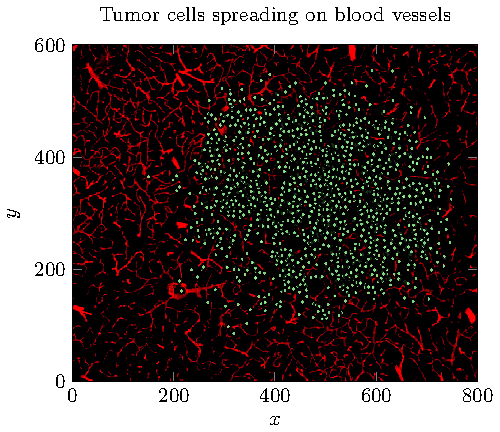
\includegraphics[width=0.4\textwidth]{Graph.pdf}
  \caption*{}
\end{wrapfigure} 
\indent In order to quantify the accuracy of our approach, we will be using a tool in mathematics called the Wasserstein Distance, which measures the distance between functions or data sets, and thereby provides us insight into the improvement that our approach to modeling stochastic systems offers. We will collaborate with
Dr.\ Pedro Lowenstein, a professor of Neurosurgery at the University of Michigan, to obtain data on cancer growth in mice. We will use the Wasserstein Distance to compare the experimental data, the predictions made by the Brownian motion approach, and the predictions made by the deterministic approach.  We seek to understand how the number of particles used in the Brownian motion approach affects the accuracy of our approximation of the biological data. More specifically, we will propose an algorithm that will determine the number of particles necessary to get within a desired error using the Brownian motion approach. 

\indent During a summer research project, completed under Dr.\ Anne Gelb, I studied the use of statistical algorithms to improve Fourier edge detection in the presence of corrupted data. Specifically, Dr.\ Gelb and I derived an algorithm for reconstructing MRI images that is twice as accurate as previous methods available to the medical community. By working with Dr.\ Gelb, I developed an interest in using statistical tools to study relevant problems in biology. During the summer of 2016 I participated in two summer research programs that provided me with the interest and background necessary to successfully complete my Origins Project research. My first project was at the University of California, Santa Barbara, where I took a series of graduate courses on differential equations in random media, biological modeling of living systems, and statistical approximations of biological processes. Through conversations with professors and graduate students from Princeton, Stanford, UC Berkeley and others, I learned about cutting-edge research at the intersection of biology and statistics and will apply these techniques in my Origins Project research.\\
\indent In my second project, I was selected as one of three from over 300 undergraduates to participate in a research experience at San Diego State University. There I studied the convergence behavior of statistical algorithms used in linear regression models. Specifically, my advisor Dr.\ Rom\'{a}n and I proposed the first algorithm for concrete convergence bounds for the error of a Gibbs sampler in a Bayesian linear regression model. These results will be submitted for publication in October. This research experience taught me the tools to complete statistical convergence analysis, and I will use similar tools to study the convergence behavior of the approximation to complex systems using Brownian-type motion. \\
\indent To successfully complete this research, I will need an advanced grasp of real analysis, probability theory, and numerical analysis. I have taken a course on numerical methods with Dr. Motsch, and I have enrolled in graduate courses in real analysis, distribution theory, and stochastic processes. In these courses I will obtain the tools necessary to analyze papers relating to my work with Dr Motsch, as well as make meaningful contributions to the field. In the Spring I will finish the graduate sequence in real analysis and probability theory, creating a solid theoretical foundation that I will use in my research.\\
\indent Developing accurate statistical algorithms for understanding stochastic complex systems is one of the largest problems in modern biological sciences, and the opportunity to study this type of problem has been my main focus during my undergraduate career. In addition to contributing to the field of computational biology, I hope to motivate theoretical mathematicians and statisticians to solve problems of interest in applied fields, bridging the gap between the two communities.
Indeed, the Wasserstein distance might also be successfully applied to problems in computer science and chemistry. In addition to significantly adding to my knowledge in statistics and computational mathematics, I hope this research project will start a larger discourse on the use of statistical algorithms, specifically Brownian motion, in biology, chemistry, and other applied fields. \\
\indent The Origins Project represents an avenue towards galvanizing an interest among pure mathematicians and statisticians in using theoretical tools to study problems of interest in biology. With the Origins Project’s Undergraduate Research Scholarship, I will have the opportunity to demonstrate the utility of mathematics and statistics in computational biology. By capturing the stochastic behavior of biological processes that govern the development of infectious diseases and our place in the universe, my research will shed light on the origin and future of humanity.


% { (alternative: {\color[rgb]{.8,0,0} By scrutinizing the role of stochastic behavior in biological processes that govern... })


 





\end{document}